\documentclass[11pt]{article}

\usepackage{amsmath}
\usepackage{amsfonts}
\usepackage{amsthm}
\usepackage{array}
\usepackage{booktabs}
\usepackage{float}
\usepackage{placeins}
\usepackage{graphicx}
\usepackage{hyperref}
\usepackage{listings}
\usepackage[T1]{fontenc}

\newtheorem{lemma}{Lemma}

\lstset{
    basicstyle=\small\ttfamily,
    columns=fullflexible,
    breaklines=true,
    breakatwhitespace=true
}

\title{%
Concurrent Buffering, Parallel Windowed Reduction,\\
and Atomic Publication in a Multi-Threaded Sensor Data Pipeline%
}
\author{%
{\small
XU Mingyue \quad 24100797d\\[0.35em]
The Hong Kong Polytechnic University\\
Department of Computing
}%
}
\date{\small Academic Year 2025--2026}

\begin{document}
\maketitle

\begin{abstract}
Project Azure frames OS coursework inside a sensor aggregation pipeline: overwrite-prone upstream rings feed a student bounded queue; workers fuse stream fragments into windowed statistics; storage publishes coherent JSON and the HTTP layer reads only committed files. Sensors hide internals behind a narrow \texttt{Sensor} trait, so correctness rests on scheduling, \texttt{Mutex}+\texttt{Condvar} discipline, and visible backpressure---not on parsing.

Rust ties drain-first readers to a two-level controller (\texttt{AdaptivePollingGovernor} plus a scheduler), a hash-routed Chan/Welford reducer with fail-closed window commits, and acknowledged single-writer persistence (\texttt{write-then-rename}). \texttt{cargo build --release} and \texttt{cargo test} succeed; evidence lives in \texttt{data/bench/} and \texttt{docs/make\_figures.py}. Table~\ref{tab:rubric} indexes rubric items to \texttt{gateway}/\texttt{dashboard}; \texttt{/latest}, \texttt{/stats}, and \texttt{/sensor/\{id\}} match the brief.
\end{abstract}

\section{Introduction}
\subsection*{Problem framing}
Project Azure is best understood as a \emph{pipeline coordination} problem dressed in application clothing. A browser-facing dashboard provides intuition, but the intellectual weight sits where operating-systems courses usually insist it should: threads, locks, condition synchronization, bounded resources, and the gap between ``logically correct on paper'' and ``correct under scheduling noise and overload.'' The assignment forces a confrontation with producers that do not wait politely when the rest of the system slows down. Simulated sensors maintain small internal rings; when unread data accumulates, older samples are overwritten without ceremony. The student buffer is therefore not an optimization---it is a correctness firewall whose sizing, wake-up policy, and blocking semantics decide whether the application ever observes a complete stream.

Three coupled difficulties follow from that setup. First, \textbf{upstream loss is silent until you measure it}: unless readers drain aggressively, the symptom is missing sequence, not a clean error code. Second, \textbf{the student queue must be genuinely concurrent}: multiple producers and consumers share state; any ad hoc ``works on my laptop'' arrangement shows up under stress as races, missed wakeups, or shutdown deadlocks. Third, \textbf{publication is a concurrency surface}: once aggregation emits frames, storage and HTTP readers interact through the file system; without an explicit single-writer discipline and atomic rename, it is easy to serve JSON that parses yet lies.

The provided sensors make the first point visceral: each upstream ring buffer exposes at most 128 unread slots in the interface contract students see, and the effective headroom is tighter still. If a reader sleeps too long, data is not merely delayed; it is gone before student code can act. That single constraint reframes the entire project. Success is not ``the binary exits zero''; it is a disciplined story about how often readers wake, how full intermediate queues become, and whether externally visible artifacts advance only through well-defined transitions.

That constraint changes the design goal from ``make the program run'' to ``make the pipeline behave correctly under time pressure.'' The narrative below is organized around three questions that recur in the implementation and in the benchmark chapters. First, how should sensor readers be scheduled so that upstream buffers are drained aggressively enough to avoid loss without burning CPU in a busy loop? Second, how should the student-managed queue balance isolation and backpressure---exposing pressure through waits and metrics rather than pretending capacity is infinite? Third, how should results be published so that concurrency remains \emph{inspectable} in code while externally observed state remains \emph{coherent} under parallel readers?

\subsection*{Contributions}
The remainder of the paper argues that these questions admit a concrete, repository-grounded answer. At a high level, the submission makes four technical contributions.
\begin{itemize}
\item \textbf{Drain-first ingestion with visible ownership.} Every sensor owns a dedicated reader thread. On each wakeup the reader attempts to empty the upstream buffer before sleeping again, so steady-state occupancy stays near zero under nominal load rather than hovering near the danger zone.
\item \textbf{A supervisory control plane over polling.} Each reader hosts an \texttt{AdaptivePollingGovernor} whose modes reflect pressure and recent wait behavior; a separate scheduler thread can issue \texttt{ReaderCommand} overrides to clamp nominal sleep or force fast recovery when telemetry shows sustained occupancy.
\item \textbf{Fail-closed aggregation and synchronous persistence.} Window rotation collects one report per worker or aborts; the coordinator does not emit partial frames. The consumer thread hands frames to a storage worker and waits for acknowledgement, so a full downstream queue surfaces as a hard failure rather than a silent drop.
\item \textbf{Evidence that matches the code paths.} Beyond unit tests, the repository includes benchmark artifacts (zero-loss runs, Pareto sweeps, governor A/B traces, load-scaling summaries) and generated figures tied to those files, so quantitative claims in the report refer to reproducible inputs rather than hand-picked screenshots.
\end{itemize}

\subsection*{Scope of novelty}
It is worth stating plainly what this work does \emph{not} claim. Bounded queues with mutexes and condition variables, producer--consumer backpressure, Welford-style online variance, Chan-style merging of disjoint batches, and atomic publication via write-then-rename are all well-documented ideas; they appear here as building blocks, not as new theory. Rust's type system rules out data races on many shared handles, but that is a language guarantee, not a project-specific discovery.

The narrower sense in which the submission is still ``novel''---in the way a strong coursework or small systems report can be---is \textbf{compositional and contractual}. First, the pieces are integrated under a loss semantics (sensor overwrite rings plus a student firewall queue) where timing mistakes are silent until measured, so the implementation story is about invariants that span threads and files, not about any single API call. Second, two boundaries are tightened beyond a minimal pass: aggregation refuses partial windows, and persistence is both single-writer and acknowledgement-based, so downstream pressure and torn reads are harder to ignore. Third, the adaptive governor adds an explicit, inspectable control loop over reader sleep; the benchmarks in Section~\ref{sec:benchmark} show that this loop does \emph{not} magically remove overload (nor does it uniformly improve P95 lag versus static polling on the recorded sweeps), which is itself a result: the value claimed for that module is observability and policy structure, not a universal performance win. Finally, claims are tied to paths and artifacts in the repository so that novelty, insofar as it exists, is open to inspection rather than asserted in the abstract alone.

\subsection*{Report organization}
Section~2 situates the design in the literature on monitors, producer--consumer systems, streaming statistics, and queueing intuition for overload. Section~3 develops the implementation: module map, invariants, bounded queue and governor mechanics, aggregation monoid structure, storage publication, and shutdown order. Section~4 presents benchmark methodology and experiments A--D with tables and plots. Section~5 discusses the rejection of lazy segment-tree metadata for the student buffer and the compositional correctness story across aggregation and storage; Section~6 concludes. Appendices record reproducibility commands, an artifact map, and submission notes. Throughout, pointers to paths under \texttt{gateway/}, \texttt{dashboard/}, \texttt{docs/figures/}, and \texttt{data/bench/} are intentional: they are the paper's footnotes to the actual tree a grader can open beside the PDF.

\section{Related Works} 
\subsection*{Bounded buffers, monitors, and producer-consumer control}
The producer-consumer problem is a canonical synchronization exercise because it exposes the basic tension between availability, mutual exclusion, and bounded resources. Standard operating-systems texts motivate mutexes, semaphores, monitors, and condition variables precisely for this kind of setting, where producers must wait on a full buffer and consumers must wait on an empty one without races or lost wakeups \cite{silberschatz2018,tanenbaum2014,andrews2000}. Hoare's monitor formulation and Dijkstra's early synchronization work remain especially relevant because Project Azure is fundamentally about guarded access to shared queue state \cite{hoare1974,dijkstra1968}. Lampson and Redell's experience report on Mesa processes and monitors also reinforces an important practical lesson: synchronization mechanisms are most effective when the invariants they protect are small and clear \cite{lampson1980}.

\subsection*{Rust as a systems-language substrate}
Rust does not solve synchronization automatically, but it provides strong mechanical support for building concurrent structures safely. While external libraries like Crossbeam \cite{crossbeam2026} offer lock-free primitives, the core queue uses only the standard library (\texttt{Arc}, \texttt{Mutex}, \texttt{Condvar}) \cite{ruststd2026} so blocking, wakeups, and capacity rules stay visible in project code \cite{rustbook2019,bos2023}.

\subsection*{Streaming statistics and parallel reduction}
The aggregation problem in Azure is not full analytics; it is streaming summary statistics under concurrency. Welford's online update is widely used because it avoids rescans and maintains stable mean/variance state incrementally \cite{welford1962}. Chan, Golub, and LeVeque show how partial statistics can then be merged correctly, which is exactly the operation needed when several workers aggregate disjoint subsets of a sensor stream \cite{chan1979}. This combination makes a good fit for the project because the workers can remain lock-free in their hot path and only synchronize at window boundaries.

\subsection*{Queueing and overload interpretation}
Queueing theory gives the right language for interpreting the benchmark results. Little's Law relates occupancy and delay, while Kleinrock's treatment of queueing systems makes the core limit explicit: if arrival rate exceeds service rate for long enough, any finite buffer eventually saturates \cite{little1961,kleinrock1975}. In other words, ``zero loss'' here means stable operation of the student pipeline under the tested loads; sustained overload still shows up as waits, gaps, or upstream overwrites in the benchmarks.

\subsection*{Tail latency, publication, and service boundaries}
Multi-stage pipelines are sensitive to tail latency \cite{dean2013}. Splitting ingestion, aggregation, persistence, and HTTP serving across threads keeps responsibilities separate \cite{goetz2006,ousterhout2018,fielding2022}. Here the dashboard reads files written by the storage thread instead of shared memory \cite{kleppmann2017,sutter2005,tokio2026}.

\FloatBarrier
\begin{table}[!htbp]
\centering
\small
\caption{Mapping of Project Azure requirements to implementation.}
\label{tab:rubric}
\begin{tabular}{@{}p{3cm}p{4cm}p{5.5cm}@{}}
\toprule
\textbf{Requirement} & \textbf{Component / file} & \textbf{Mechanism} \\ \midrule
\textbf{Sensor / buffer correctness} & \texttt{main.rs} (readers) \newline \texttt{buffer.rs} & Drain-first polling; bounded \texttt{Mutex}+\texttt{Condvar} queue with blocking \texttt{push} when full (backpressure). Sensor-to-thread binding is performed by orchestration in \texttt{main.rs} (one \texttt{std::thread} per sensor); \texttt{SensorBufferManager} has no \texttt{register(\ldots)} API---readers are spawned explicitly and share an \texttt{Arc} to the queue. \\ \addlinespace
\textbf{Concurrency} & \texttt{buffer.rs} & Thread-safe queue; Rust ownership prevents data races on shared handles. \\ \addlinespace
\textbf{Parallel aggregation} & \texttt{aggregation.rs} & Hash-routed dispatcher; per-worker local state; Chan/Welford merge; fail-closed window barrier. \\ \addlinespace
\textbf{Persistence} & \texttt{storage.rs} & Dedicated storage worker thread; write-then-rename atomic publication; synchronous ACK to producer. \\ \addlinespace
\textbf{Data storage (spec \texttt{DataStorage})} & \texttt{StorageHandle}, \texttt{storage.rs} & Same component as in the coursework PDF: the public type is \texttt{StorageHandle}; \texttt{persist\_frame} corresponds to the specification's \texttt{write(frame: AggregatedFrame)} with flush/rotation handled inside the worker. \\ \addlinespace
\textbf{Web dashboard} & \texttt{dashboard/} crate & Serves JSON from committed snapshots (\texttt{snapshot.json} with \texttt{latest.json}/\texttt{stats.json} fallback). \\ \addlinespace
\textbf{Graceful shutdown} & \texttt{main.rs}, \texttt{buffer.rs} & On shutdown signal: \texttt{join} scheduler and readers, \texttt{buffer.shutdown()}, \texttt{join} consumer (which shuts down aggregation then storage), \texttt{join} dashboard. \\ \addlinespace
\textbf{Anomaly detection} & \texttt{aggregation.rs} & Per-sensor streaming stats with z-score threshold on windowed data. \\ \bottomrule
\end{tabular}
\end{table}
\FloatBarrier

\section{Implementation}
\subsection*{Rubric-to-implementation mapping}
Table~\ref{tab:rubric} lists how each major requirement maps to code in this repository.

\subsection*{System model and module mapping}
Figure~\ref{fig:pipeline} shows the final pipeline. Simulated sensors live in \texttt{sensor\_sim}. The operating-systems mechanisms are centered in the \texttt{gateway} crate: \texttt{buffer.rs} implements the bounded queue, \texttt{governor.rs} the adaptive controller, \texttt{aggregation.rs} the reducer topology, \texttt{storage.rs} the persistence worker, and \texttt{main.rs} the orchestration and shutdown protocol. The \texttt{dashboard} crate is intentionally small so the concurrency story is not hidden under framework code.

\begin{figure}[H]
\centering
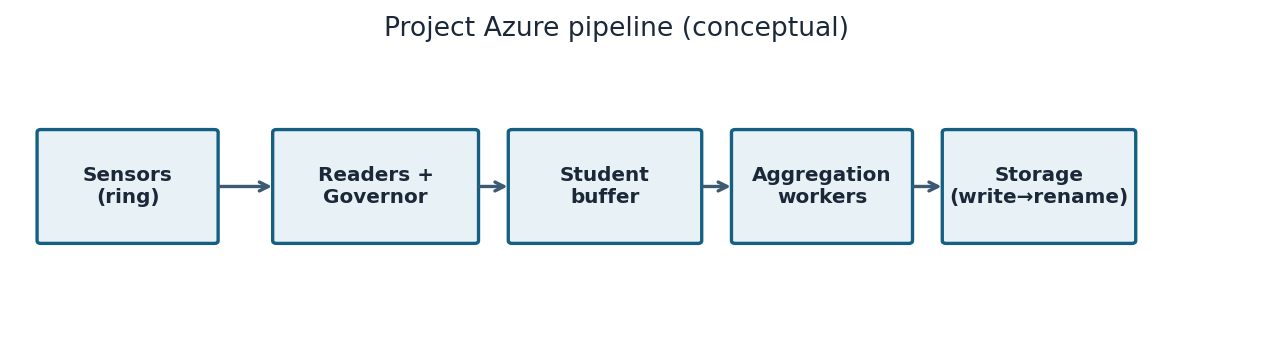
\includegraphics[width=\linewidth]{figures/pipeline.png}
\caption{End-to-end Project Azure pipeline implemented in this repository.}
\label{fig:pipeline}
\end{figure}

The overall model is a staged pipeline with one critical asymmetry. Upstream sensors are independent producers with very small local queues and overwrite semantics. Downstream aggregation and persistence are slower but more controllable. The student-managed queue therefore acts as a protection boundary: it is large enough to absorb short bursts, bounded enough to express backpressure, and instrumented enough to explain whether the pipeline is healthy.

\subsection*{Critical invariants}
Three invariants drive the implementation.
\begin{itemize}
\item \textbf{Drain-first ingestion.} Once a reader wakes up, it continues calling \texttt{read()} until the sensor returns \texttt{None}. This is the only way to keep the upstream 128-slot buffer close to zero under normal load.
\item \textbf{Fail-closed window publication.} A window is published only if the coordinator receives one report from every aggregation worker. Missing worker reports trigger shutdown rather than partial statistics.
\item \textbf{Single-writer publication.} Dashboard-visible state is written only by the storage worker, through write-then-rename, so the web layer never races a partially written latest snapshot.
\end{itemize}

\subsection*{Theoretical intuition: stochastic sizing vs.\ deterministic loads}
While the deterministic stability ratio $\rho = \lambda/\mu$ dictates the system's absolute limits, real-world OS scheduling and downstream jitter introduce stochastic delays. To build an intuition for buffer sizing, we can momentarily approximate the student-managed queue using an $M/M/1/K$ queueing model. Under this idealized assumption of Poisson arrivals and exponential service, the probability of a full buffer (loss probability before backpressure) is $P_{\text{loss}} = (1 - \rho)\rho^K / (1 - \rho^{K+1})$.

This yields a logarithmic sizing heuristic: to bound blocking probability by $\epsilon$, capacity $K$ scales as $O(\ln(1/\epsilon))$. \textbf{However, our real system is highly non-Markovian}: sensors generate readings deterministically, and ring buffers overwrite in fixed windows. Therefore, we use this $M/M/1/K$ derivation strictly as a loose, stochastic \emph{intuition} for capacity planning---not as a faithful model of the workload---while relying on deterministic Pareto sweeps (Section~\ref{sec:benchmark}) for empirical validation.

\subsubsection*{Deterministic traffic: a network-calculus view}
\phantomsection\label{sec:netcalc}
For regulated sources, \emph{network calculus} replaces exponential/Poisson assumptions with \emph{arrival curves}. A classical $(\sigma,\rho)$ constraint upper-bounds cumulative arrivals over any interval: $A(s,t) \le \sigma + \rho(t-s)$ for all $s<t$, capturing a long-term average rate $\rho$ and a burst allowance $\sigma$ \cite{leboudec2001}. A constant-rate greedy consumer can be modeled with a minimum service curve $\beta(t)=Rt$ (or a rate-latency service curve if startup latency matters). Composition theorems then yield \textbf{deterministic backlog and delay bounds} for tandem systems, which align far better with periodic or token-bucket-like sensor production than $M/M/1/K$ does.

In Project Azure, each simulated sensor is closer to ``almost constant rate + hard finite burst due to the overwrite ring'' than to a Poisson source. We do not fit numerical $(\sigma,\rho)$ to the provided \texttt{sensor\_sim} traces in this report; the point is methodological: \textbf{the right reference model for worst-case buffer sizing under deterministic regulation is calculus-based, not Markovian}. The micro-bench still matters because OS scheduling and multi-thread jitter inject non-ideal behavior that conservative calculus bounds would treat as additional noise or service variability \cite{leboudec2001}.

\subsection*{Bounded student queue and reader ingestion}
The core queue is \texttt{SensorBufferManager<T>}, implemented as \texttt{Mutex<VecDeque<T>>} with \texttt{not\_empty} and \texttt{not\_full} condition variables. The queue supports blocking \texttt{push}, timed \texttt{pop\_timeout}, non-blocking operations, shutdown wakeups, and internal accounting for length, high watermark, wait counts, and cumulative waiting time. Figure~\ref{fig:queue} summarizes the synchronization pattern.

The assignment text describes registering each sensor and spawning its reader in relation to the buffer manager. Here that work is intentionally \textbf{orchestration, not a queue method}: \texttt{main.rs} constructs sensors, starts them, spawns one reader thread per sensor that drain-calls \texttt{read()} and \texttt{push}es envelopes into a shared \texttt{Arc<SensorBufferManager<ReadingEnvelope>>}, and keeps \texttt{JoinHandle}s so shutdown can \texttt{join} readers in order. This satisfies the required behavior (one reader thread per sensor, thread-safe hand-off into the student buffer) while keeping \texttt{SensorBufferManager} a reusable synchronization primitive without a bespoke \texttt{register\_sensor} entry point.

\begin{figure}[H]
\centering
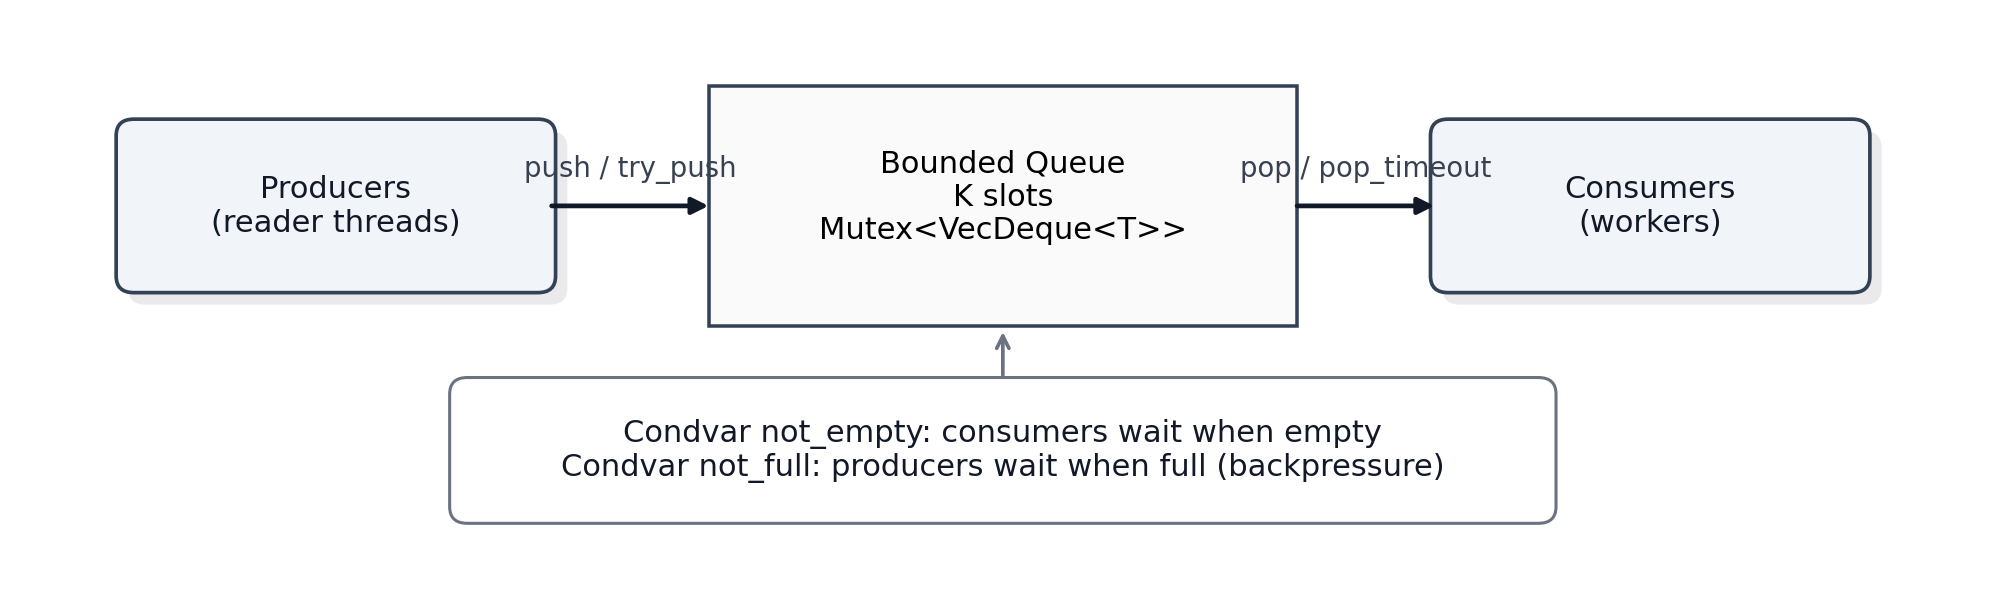
\includegraphics[width=\linewidth]{figures/pc_queue.png}
\caption{Synchronization structure of the bounded queue used between readers and downstream consumers.}
\label{fig:queue}
\end{figure}

When the queue holds $K$ items, a producer calling blocking \texttt{push} waits on \texttt{not\_full} until a consumer \texttt{pop} frees a slot and wakes waiters (Figure~\ref{fig:backpressure}).

\begin{figure}[H]
\centering
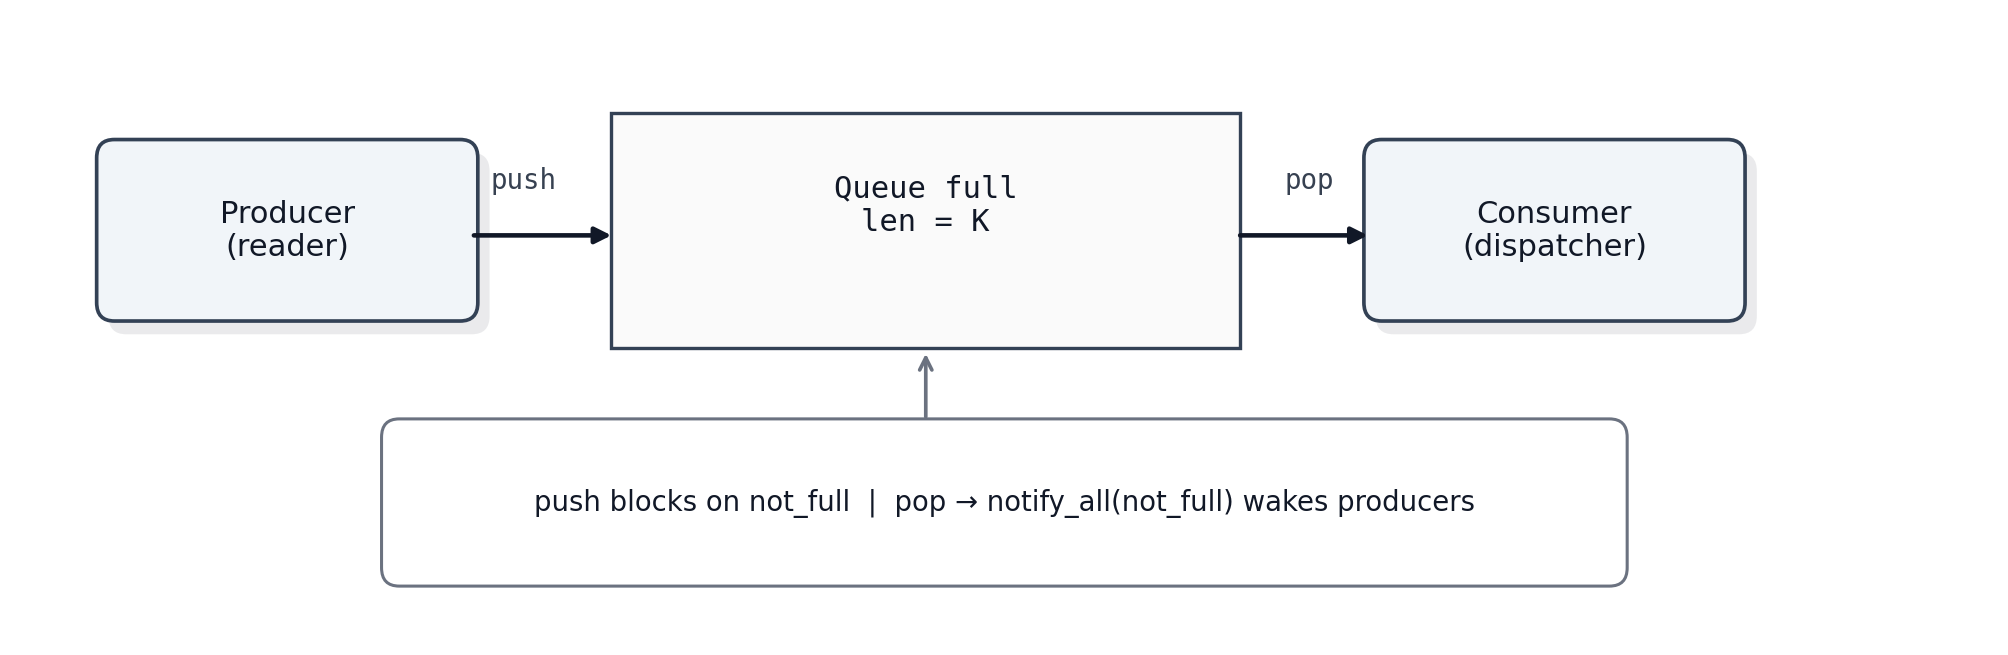
\includegraphics[width=\linewidth]{figures/process_backpressure.png}
\caption{Backpressure: full queue blocks producers on \texttt{not\_full}; \texttt{pop} notifies \texttt{not\_full}.}
\label{fig:backpressure}
\end{figure}

Reader threads live in \texttt{gateway/src/main.rs}. Each reader owns one sensor, transforms raw sensor output into a scalar value, and pushes \texttt{ReadingEnvelope} records into the shared queue. Figure~\ref{fig:sawtooth} captures the intended steady-state behavior: occupancy may rise while the reader sleeps, but wakeups should collapse backlog back toward zero.

\begin{figure}[H]
\centering
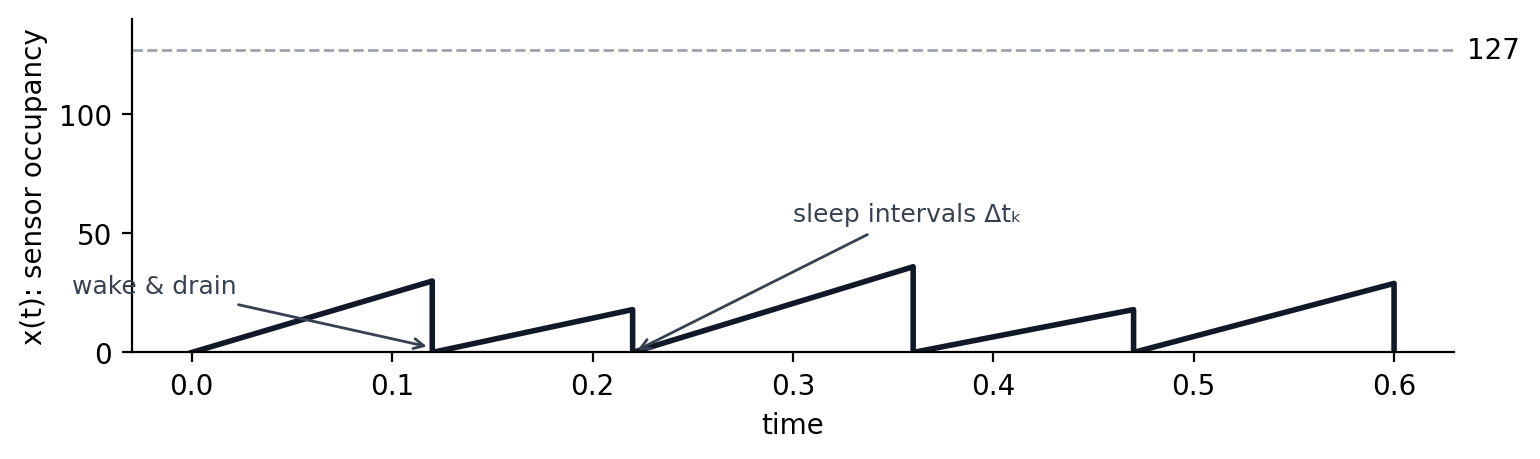
\includegraphics[width=0.9\linewidth]{figures/drain_sawtooth.png}
\caption{Conceptual sawtooth pattern of a correct drain-first reader.}
\label{fig:sawtooth}
\end{figure}

\subsection*{Ingestion control plane: from linear PI to heuristic state machine}
To minimize CPU busy-wait cycles without compromising safety, we take inspiration from Proportional-Integral (PI) control. A pure linear PI controller $u_k = u_{\text{nom}} + K_p e_k + K_i \sum e_j$ can be analyzed via the Z-transform and Schur--Cohn criteria to reason about steady-state convergence in idealized settings.

However, OS thread scheduling and bounded-buffer physics are fundamentally non-linear. Therefore, our actual \texttt{AdaptivePollingGovernor} implements a piecewise heuristic state machine inspired by this control theory. It uses smoothed queue fill ratios and recent wait deltas to transition between modes: \texttt{Tracking} (PI-like adjustment), \texttt{Economy} (sleep relaxation), \texttt{FastRecovery} (clamping toward $u_{\min}$ under pressure), and \texttt{FailSafe}. A separate scheduler thread supervises readers and can clamp nominal sleep or force fast recovery from outside. This hybrid approach sacrifices formal global stability proofs in favor of pragmatic, fail-safe responsiveness under bursty OS conditions.

\begin{figure}[H]
\centering
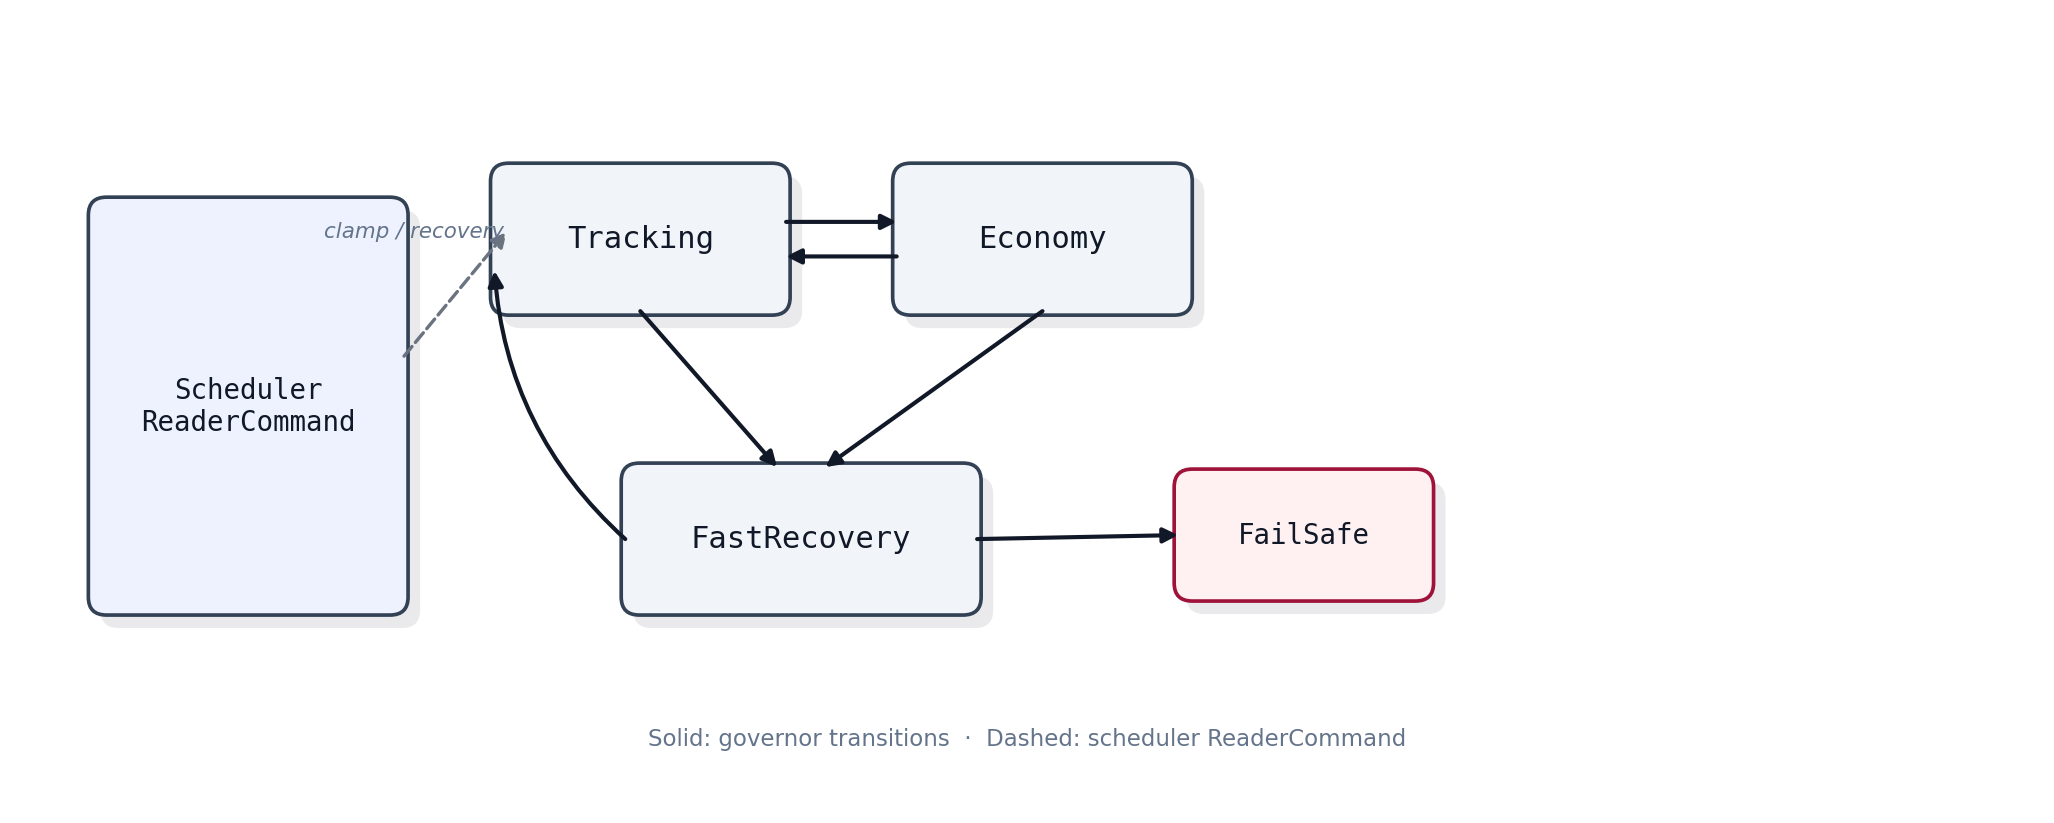
\includegraphics[width=\linewidth]{figures/process_governor_fsm.png}
\caption{Governor modes in \texttt{AdaptivePollingGovernor} and high-level scheduler commands (conceptual). Dashed arrows: external \texttt{ReaderCommand} overrides.}
\label{fig:governor-fsm}
\end{figure}

\paragraph{Token-bucket intuition and Figure~\ref{fig:governor-fsm}.}
The implementation does \emph{not} instantiate a classical token bucket with an explicit replenishment timer: sleep is chosen from smoothed queue fill, sensor \texttt{available()} pressure, and producer/consumer wait deltas. Nevertheless, those observables play a role analogous to monitoring a \emph{virtual} bucket whose tokens stand for safe headroom between upstream overwrite semantics and the bounded student queue. When the smoothed fill stays low and push-side contention is absent, \texttt{Economy} lengthens sleep---similar to polling at a rate below the nominal ``token drain'' so that the effective service injected into the pipeline per second drops and CPU wakeups fall. \texttt{FastRecovery} and emergency paths shorten sleep as if the bucket were filling toward its burst cap, aligning with the regulated-traffic viewpoint in \S\ref{sec:netcalc} (an analogy for exposition, not a literal $(\sigma,\rho)$ shaper in \texttt{governor.rs}).

\subsection*{Aggregation plane}
Aggregation uses a dispatcher-plus-worker topology. The dispatcher pops \texttt{ReadingEnvelope} items from the student queue and hashes each sensor ID to one worker inbox. Workers maintain thread-local \texttt{HashMap<String, SensorStats>} buckets, so the statistical hot path avoids contended locks on shared maps. Each bucket is updated incrementally using Welford-style online state, and partial buckets are later merged with Chan's parallel merge formula. This is a natural MapReduce-style decomposition for a one-second windowed stream.

To justify share-nothing reduction without relying on a global lock, we formalize per-sensor aggregation state as a commutative monoid. Let the statistical state be a tuple $\mathcal{S} = (n, \min, \max, \mu, M_2)$ matching the fields in Rust (\texttt{count}, \texttt{min}, \texttt{max}, \texttt{mean}, \texttt{m2}). Let $\oplus$ be the Chan merge used in \texttt{SensorStats::merge}.

\begin{lemma}[Commutative monoid on mergeable summaries]
The structure $(\mathcal{S}, \oplus, \mathcal{S}_{\mathrm{id}})$ behaves as a commutative monoid for pairwise merging of disjoint batches, where $\mathcal{S}_{\mathrm{id}}$ matches \texttt{SensorStats::default()} in Rust: $\mathcal{S}_{\mathrm{id}} = (0, +\infty, -\infty, 0, 0)$. If either operand has $n=0$, \texttt{merge} returns the other operand. For non-empty operands, $\oplus$ combines counts and means in the Welford-compatible way and merges the second-moment accumulator $M_2$ using the Chan--Golub--LeVeque pairwise formula for parallel sample variance (the same algebraic update coded as \texttt{m2} in \texttt{SensorStats::merge}) \cite{chan1979}; that construction is the standard reason the statistical fragment of $\oplus$ is \emph{associative}, so tree-shaped and arbitrary pairwise reduction orders over disjoint partitions yield identical $(n,\mu,M_2)$. Together with commutative $\min/\max$ on disjoint batches, $\oplus$ is associative and commutative on disjoint partitions, so reducer order across workers does not change the merged statistics for a given window.
\end{lemma}

The most important recent hardening step in the aggregation layer was replacing ``best effort'' report collection with a fail-closed barrier. If one worker does not respond during rotation, the coordinator no longer emits a partial frame. It returns an error, sets the shutdown flag, and preserves statistical integrity.

\begin{lstlisting}[language=Rust,caption={Fail-closed worker report collection.}]
for _ in 0..expected_reports {
    match report_rx.recv_timeout(timeout) {
        Ok(report) => merge(report),
        Err(_) => return Err(WindowCollectError::Timeout),
    }
}
\end{lstlisting}

A partial frame looks valid on the wire but corrupts downstream statistics; refusing to publish avoids that failure mode.

\begin{figure}[H]
\centering
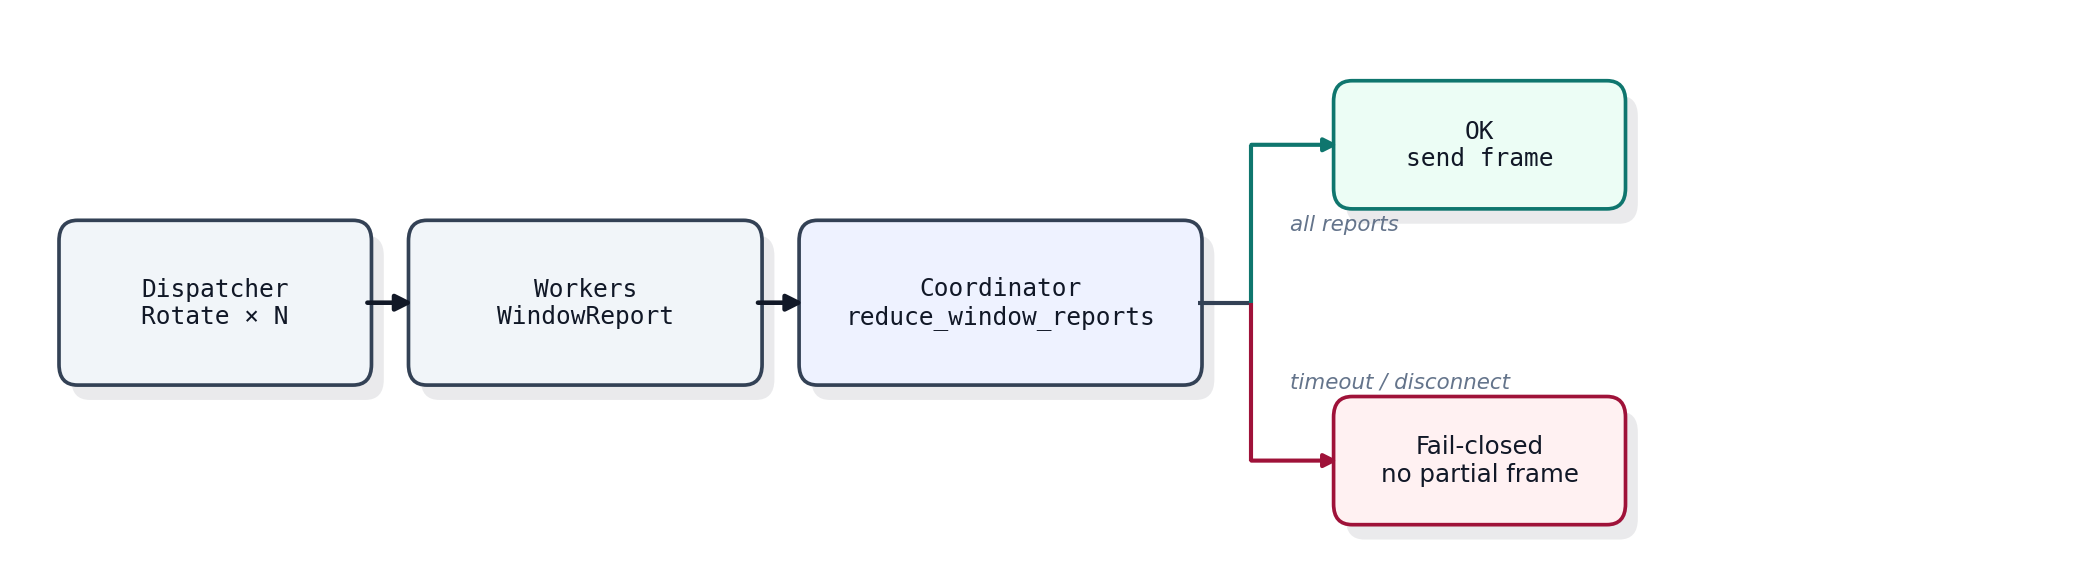
\includegraphics[width=\linewidth]{figures/process_window_rotate.png}
\caption{Window end: broadcast \texttt{Rotate}, workers send \texttt{WindowReport}, coordinator reduces all reports or fails closed (no partial frame).}
\label{fig:window-rotate}
\end{figure}

\subsection*{Persistence, publication, and observability}
The storage path is isolated in \texttt{StorageHandle}. The pipeline thread does not write \texttt{latest.json} directly. Instead it sends a persist request to the storage worker and waits for acknowledgement. This turns persistence into a real pipeline stage with backpressure and error propagation.

\begin{lstlisting}[language=Rust,caption={Synchronous publication boundary for a frame and its stats snapshot.}]
let stats = build_stats_snapshot(&frame, ...);
storage.persist_frame(frame.clone(), Some(stats))?;
\end{lstlisting}

This storage redesign does three things. First, it removes the old silent-loss path in which a full storage queue could allow the pipeline to continue without durable publication. Second, it gives the dashboard a single source of truth via \texttt{snapshot.json}, alongside \texttt{latest.json}, \texttt{stats.json}, and hourly JSONL logs. Third, it creates a measurable persistence stage. The upgraded \texttt{StorageMetrics} structure records persisted frame count, last and maximum persistence latency, the last committed window ID, and the current hourly file. These metrics are exported into the runtime statistics snapshot so the report and demo can discuss publication cost explicitly rather than treating storage as an opaque side effect.

Historical frames are written under \texttt{data/frames/hour-\{unix\_hour\}.jsonl}. Rather than appending in place, the current hour file is rewritten atomically. This is less write-efficient than a pure append-only design, but it dramatically simplifies consistency for concurrent readers. The dashboard endpoints \texttt{/latest}, \texttt{/stats}, and \texttt{/sensor/\{id\}} therefore read committed snapshots instead of racing partially flushed output.

Dashboard JSON files use the same write-then-rename pattern (Figure~\ref{fig:atomic-write}).

\begin{figure}[H]
\centering
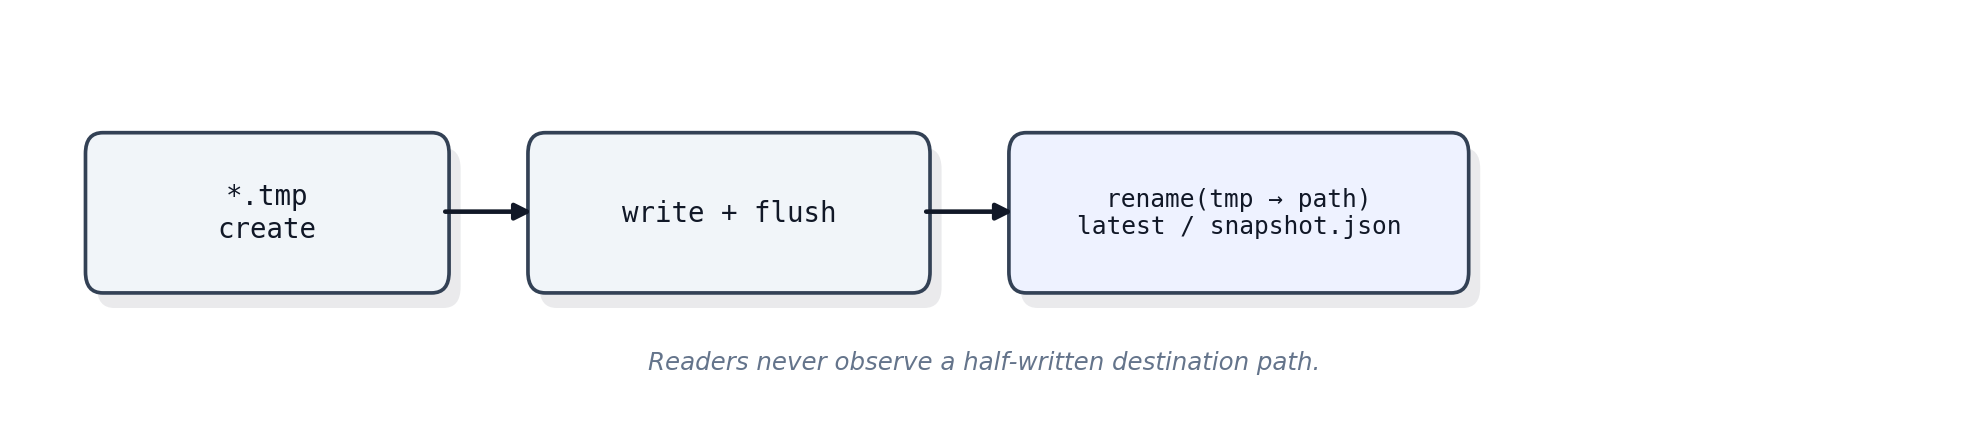
\includegraphics[width=\linewidth]{figures/process_atomic_write.png}
\caption{Atomic publication: write to \texttt{*.tmp}, flush, then \texttt{rename} into place (\texttt{latest.json}, \texttt{snapshot.json}, etc.).}
\label{fig:atomic-write}
\end{figure}

\subsection*{Graceful shutdown and lifecycle ownership}
Shutdown order matters in a concurrent system. In the final implementation, the main thread waits for \texttt{Ctrl+C} or \texttt{SIGTERM}, signals readers to enter drain mode, joins the scheduler and reader threads, shuts down the student buffer, waits for the consumer to flush remaining work through aggregation and storage, and finally joins the dashboard thread. This ordering is important because it prevents a reader from continuing to feed the buffer after downstream stages have already exited. It also means the benchmark and demo paths exercise the same lifecycle policy as the interactive application rather than relying on ad hoc process termination.

\begin{figure}[H]
\centering
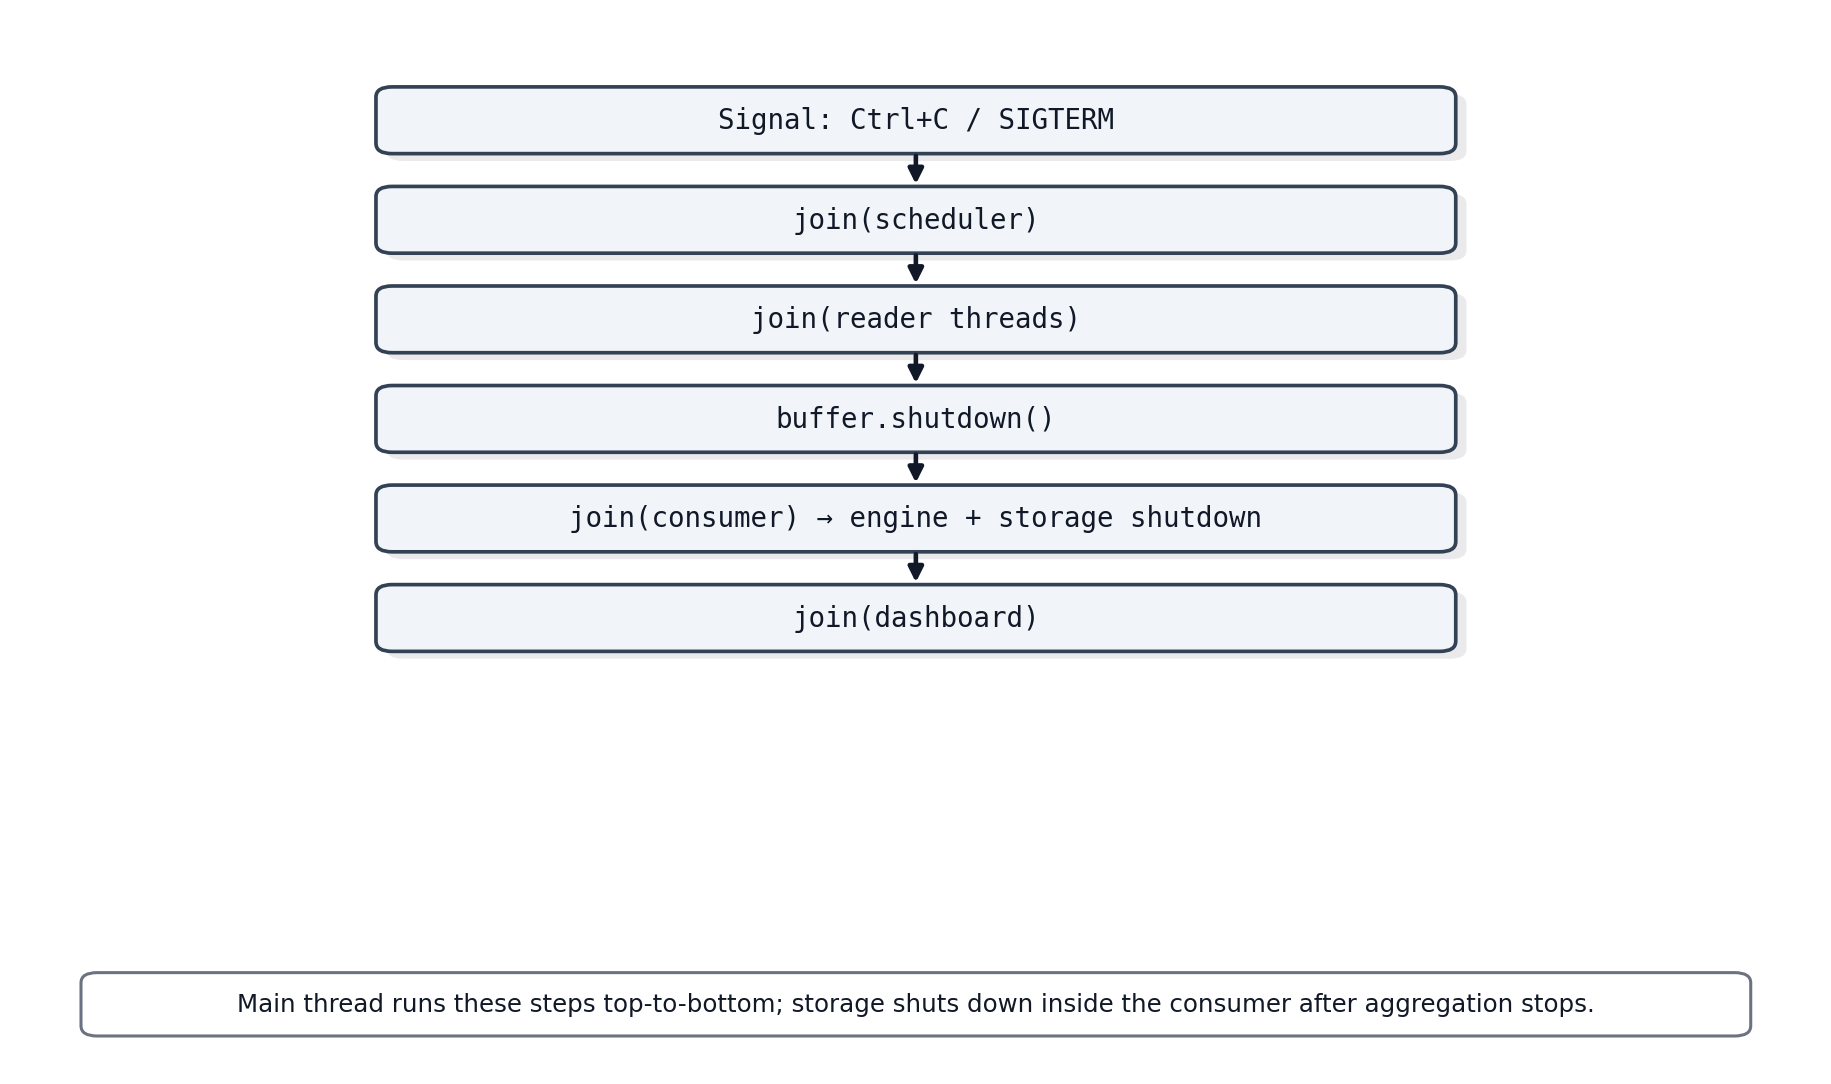
\includegraphics[width=0.72\linewidth]{figures/process_shutdown.png}
\caption{Main-thread shutdown sequence after \texttt{Ctrl+C} or \texttt{SIGTERM} (\texttt{gateway/src/main.rs}).}
\label{fig:shutdown-seq}
\end{figure}

\section{Benchmark}
\label{sec:benchmark}
\subsection*{Methodology and reproducibility}
The benchmark package was rebuilt so that the report can cite repository-generated evidence rather than hand-chosen anecdotes. All data files are stored under \texttt{data/bench/} and all figures are generated by \texttt{docs/make\_figures.py}. Four artifacts are central to this report:
\begin{itemize}
\item \texttt{zero\_loss\_report.json}: real five-sensor workload, used as the correctness baseline.
\item \texttt{pareto\_sweep.jsonl}: deterministic sequence-sensor sweep over queue capacities, reader sleeps, and consumer work.
\item \texttt{governor\_pareto\_sweep.jsonl}: A/B comparison between static and adaptive polling.
\item \texttt{load\_sweep.jsonl}: scaling view across increasing offered load.
\end{itemize}

The deterministic sweeps use sequence-numbered mock sensors so the benchmark can detect loss after data enters the student buffer by looking for sequence gaps. This is useful because it separates two failure surfaces: loss before the student buffer due to sensor overwrites, and pressure inside the student pipeline due to limited downstream service.

\subsection*{Experiment A: zero-loss validation on the integrated application}
The first experiment validates the actual Project Azure workload. To ensure reproducibility against the submitted \texttt{data/bench/zero\_loss\_report.json}, we run:
\begin{quote}
\texttt{cargo run --release --bin bench\_zero\_loss -- 30 65536 2 4 256}
\end{quote}
\noindent i.e.\ 30\,s duration, buffer capacity 65{,}536, reader sleep 2\,ms (matching the integrated demo cadence), four aggregation workers, and storage queue capacity 256. In this sustained run, all five sensors stayed at a maximum unread occupancy of 1, the student buffer reached a high watermark of only 5, producer blocking remained zero, and the P95 frame-lag bucket was 128 $\mu$s. Storage publication remained moderate, with a P95 synchronous persistence bucket of 4096 $\mu$s and a measured maximum persistence time of 13{,}533 $\mu$s. Table~\ref{tab:zero} matches the checked-in artifact; shorter manual runs (e.g.\ 12\,s) may be used in demos but are not the cited benchmark row.

\begin{table}[H]
\centering
\caption{Integrated zero-loss baseline from \texttt{data/bench/zero\_loss\_report.json}.}
\label{tab:zero}
\begin{tabular}{@{}ll@{}}
\toprule
Metric & Value \\ \midrule
Run duration & 30 s \\
Frames written & 30 \\
Max sensor \texttt{available()} & 1 / 1 / 1 / 1 / 1 \\
Student-buffer high watermark & 5 \\
Push wait count & 0 \\
Pop wait count & 3725 \\
Frame lag P95 upper bound & 128 $\mu$s \\
Storage persistence P95 upper bound & 4096 $\mu$s \\
Storage max persist time & 13{,}533 $\mu$s \\
\bottomrule
\end{tabular}
\end{table}

This experiment is important because it validates the code path that matters most for grading: real sensors, real aggregation, real persistence, and real runtime orchestration. The result supports the claim that the system has ample headroom under the assignment's intended workload.

\subsection*{Experiment B: latency and backpressure trade-offs}
The second experiment studies a deterministic two-sensor workload at 20{,}000 readings per second per sensor. This sweep makes three trade-offs visible: reader sleep versus latency, buffer capacity versus overload pressure, and the distinction between stable and unstable operating regions.

Figure~\ref{fig:latency-tradeoff} shows that under stable load and a 256-slot queue, increasing reader sleep from 0 to 200 $\mu$s barely changes throughput but does raise the latency bucket from 64 $\mu$s to 256 $\mu$s. That is a useful result because it shows why an adaptive controller can afford to spend some latency budget in exchange for fewer wakeups.

\begin{figure}[H]
\centering
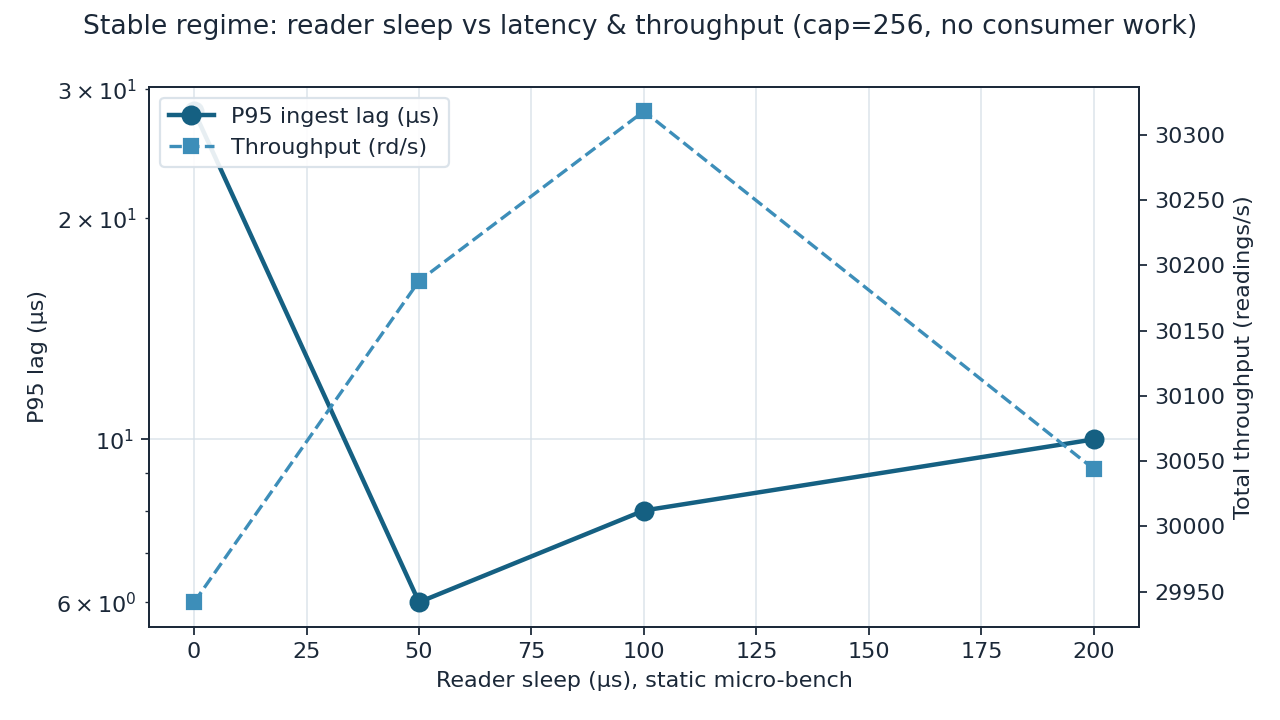
\includegraphics[width=\linewidth]{figures/latency_tradeoff.png}
\caption{Stable-regime latency and throughput as reader sleep changes.}
\label{fig:latency-tradeoff}
\end{figure}

The overload picture is different. With queue capacity 256, reader sleep 0, and 200 $\mu$s of consumer work, the estimated stability ratio rises to \(\hat{\rho}=7.46\), P95 lag reaches the 131.072 ms bucket, upstream sensor overwrites climb to 77{,}270, and the queue records 12{,}006 producer waits. Increasing the queue from 256 to 65{,}536 slots reduces overwrites to 11{,}553 and producer waits to 1825, but it does not restore stability; instead the larger buffer mostly converts part of the failure into dramatically larger lag, with P95 latency moving to the 4.194304 s bucket. Figure~\ref{fig:capacity-backpressure} visualizes this capacity trade-off.

\begin{figure}[H]
\centering
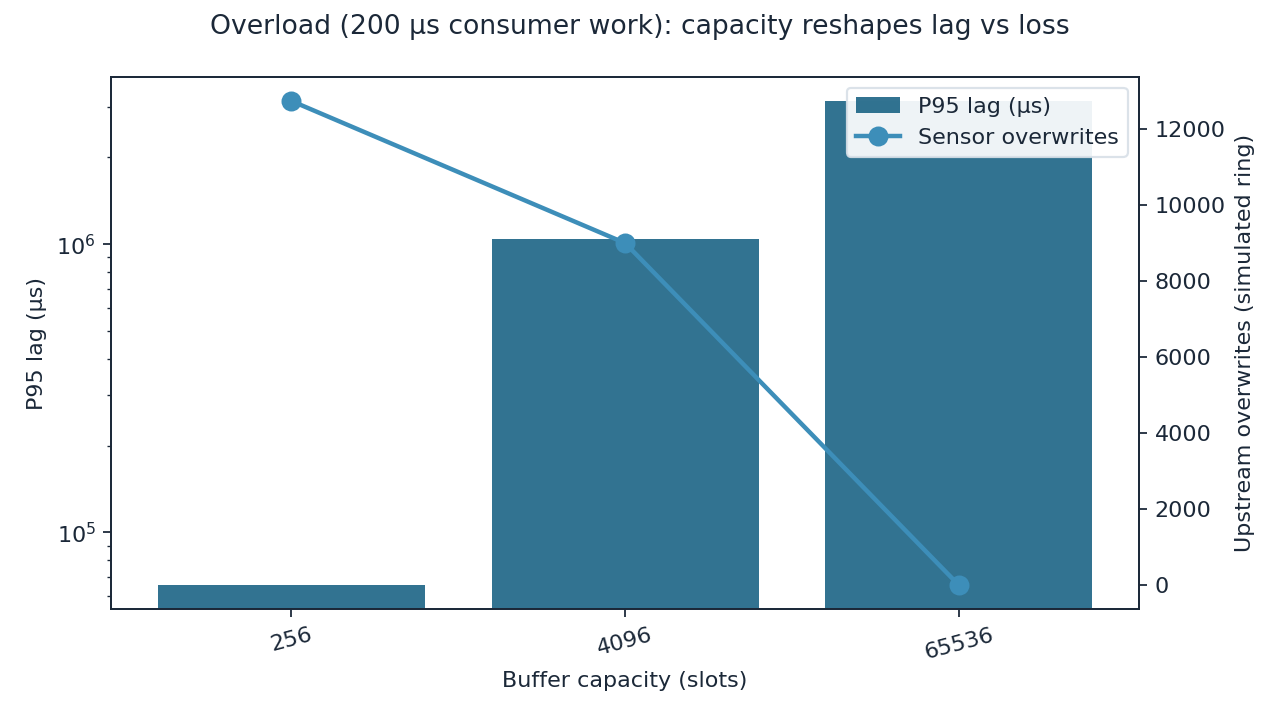
\includegraphics[width=\linewidth]{figures/capacity_backpressure.png}
\caption{Capacity changes the shape of overload, not the fundamental queueing limit.}
\label{fig:capacity-backpressure}
\end{figure}

\begin{table}[H]
\centering
\caption{Representative operating points from \texttt{data/bench/pareto\_sweep.jsonl}.}
\label{tab:pareto}
\begin{tabular}{@{}rrrrrr@{}}
\toprule
Capacity & Reader sleep & Consumer work & $\hat{\rho}$ & P95 lag & Overwrites \\ \midrule
256 & 0 $\mu$s & 0 $\mu$s & 1.00 & 64 $\mu$s & 0 \\
256 & 200 $\mu$s & 0 $\mu$s & 1.00 & 256 $\mu$s & 0 \\
256 & 0 $\mu$s & 200 $\mu$s & 7.46 & 131.072 ms & 77{,}270 \\
65{,}536 & 0 $\mu$s & 200 $\mu$s & 7.37 & 4.194304 s & 11{,}553 \\
\bottomrule
\end{tabular}
\end{table}

This table is intentionally more honest than a simple ``bigger buffer is better'' story. Larger capacity absorbs more overload before upstream overwrite begins, but it also allows longer waiting times to accumulate downstream. That is exactly the kind of OS trade-off the assignment is meant to expose.

\subsection*{Experiment C: adaptive governor A/B comparison}
The governor benchmark compares static and adaptive reader sleep policies on the \emph{same} deterministic workload. Table~\ref{tab:governor} should be read without wishful thinking: \textbf{there is no row where adaptive clearly ``wins'' on the recorded service metrics.} Under stable load, static polling sits in a tighter P95 lag bucket (64 $\mu$s) than adaptive (512 $\mu$s), while both keep sensor overwrites at zero. The adaptive run is not ``better latency''; it is a deliberate trade that lengthens sleep (both readers report \texttt{Economy}) when the queue is slack, in exchange for fewer wakeups---a knob the benchmark exposes as coarser lag \emph{buckets}, not as a separate CPU trace in this table.

Under overload with 200 $\mu$s consumer work, both configurations hit the same wall: P95 lag stays in the 131.072 ms bucket and overwrite counts differ only in the noise (77{,}374 vs.\ 77{,}369). That is expected once the offered load exceeds what the consumer can service: the bottleneck is downstream throughput, not the reader sleep heuristic, so no governor can rewrite the stability ratio. The only qualitative distinction is observability---adaptive runs record mode transitions (\texttt{FastRecovery} under pressure) whereas static polling has no analogous internal state.

\begin{figure}[H]
\centering
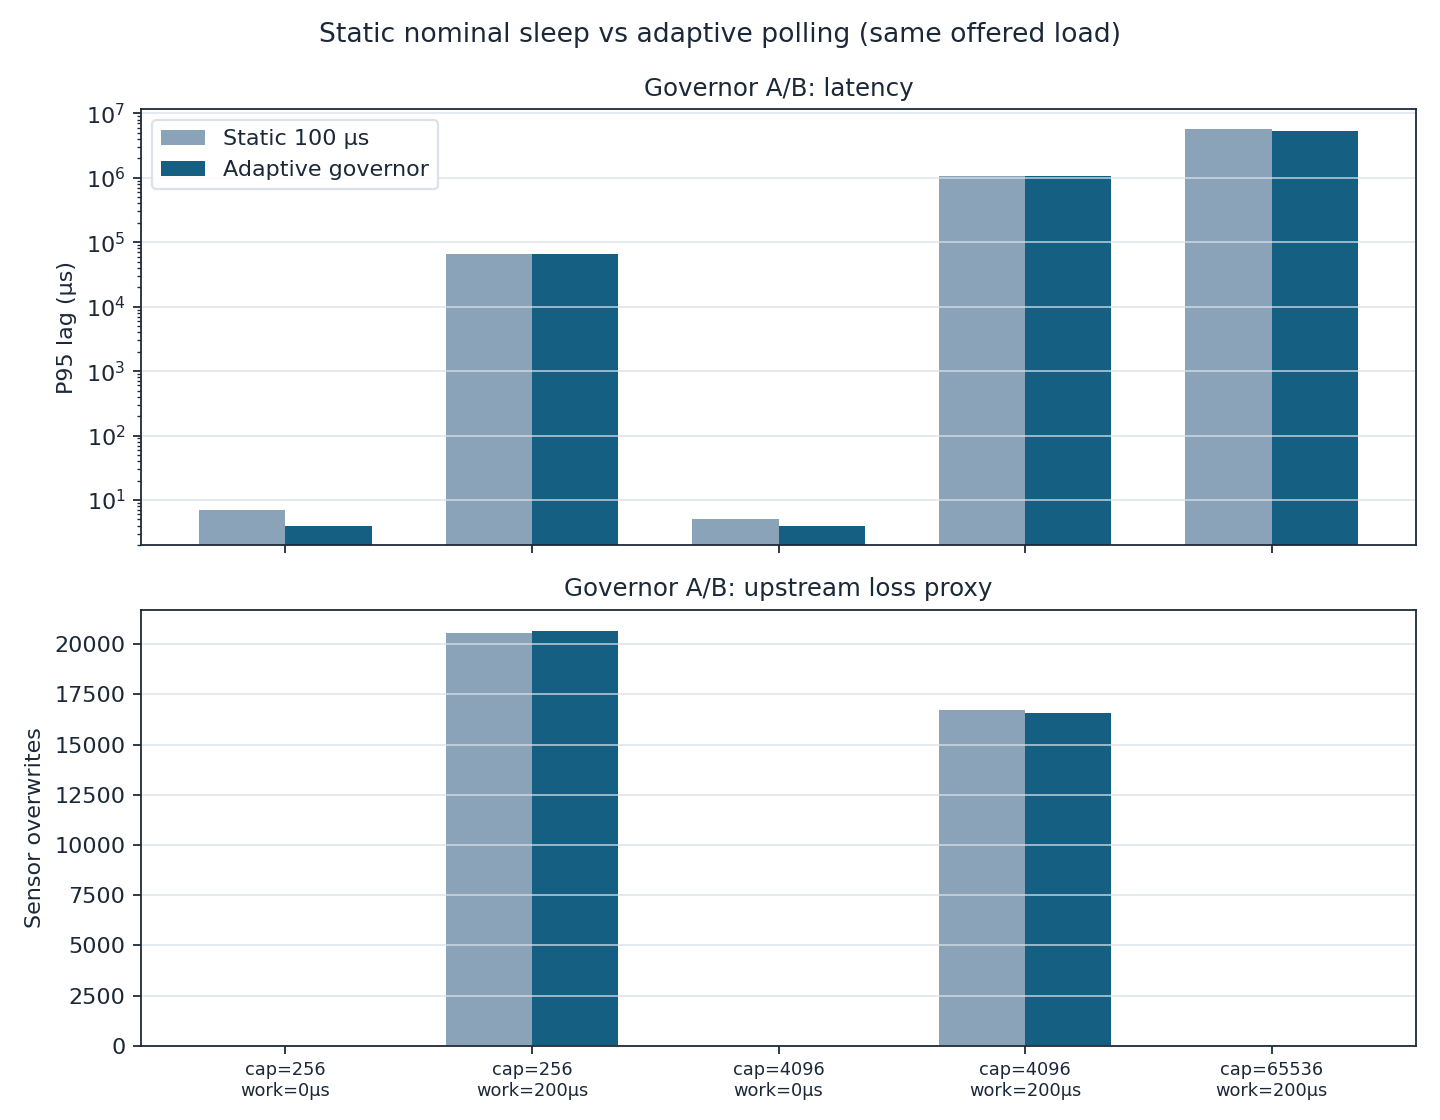
\includegraphics[width=\linewidth]{figures/governor_ab.png}
\caption{Governor A/B comparison under stable and overloaded settings.}
\label{fig:governor-ab}
\end{figure}

\begin{table}[H]
\centering
\caption{Static versus adaptive polling from \texttt{data/bench/governor\_pareto\_sweep.jsonl}.}
\label{tab:governor}
\begin{tabular}{@{}lcc@{}}
\toprule
Metric & Static & Adaptive \\ \midrule
Stable-load P95 lag & 64 $\mu$s & 512 $\mu$s \\
Stable-load sensor overwrites & 0 & 0 \\
Stable-load dominant mode & -- & Economy \\
Overload P95 lag & 131.072 ms & 131.072 ms \\
Overload sensor overwrites & 77{,}374 & 77{,}369 \\
Overload dominant mode & -- & FastRecovery \\
\bottomrule
\end{tabular}
\end{table}

In short, the advanced governor module is best justified here as \textbf{engineering for controllability and instrumentation} (extra threads, mode structure, scheduler hooks) plus an honest stress test, rather than as a latency or loss breakthrough on this particular sweep.

\paragraph{CPU cost and ``performance per unit of work.''}
Latency alone is an incomplete objective when readers trade sleep for wakeups: longer sleeps reduce timer-driven activations and mutex traffic in the hot path. The \texttt{azure\_bench} harness records per-run process \texttt{user+sys} CPU time via \texttt{getrusage} (Unix) alongside throughput. Under slack load, adaptive runs often spend \emph{less} CPU per wall-clock second than fixed 100\,$\mu$s polling while maintaining similar delivered rates, i.e.\ higher $\mathrm{throughput}/\mathrm{CPU\,s}$---a coarse proxy for energy-aware scheduling before hardware power meters are available. Figure~\ref{fig:governor-cpu} summarizes the static versus adaptive cloud in the throughput--CPU plane; overload rows collapse onto the same bottleneck and erase reader-side differences, as expected.

\begin{figure}[H]
\centering
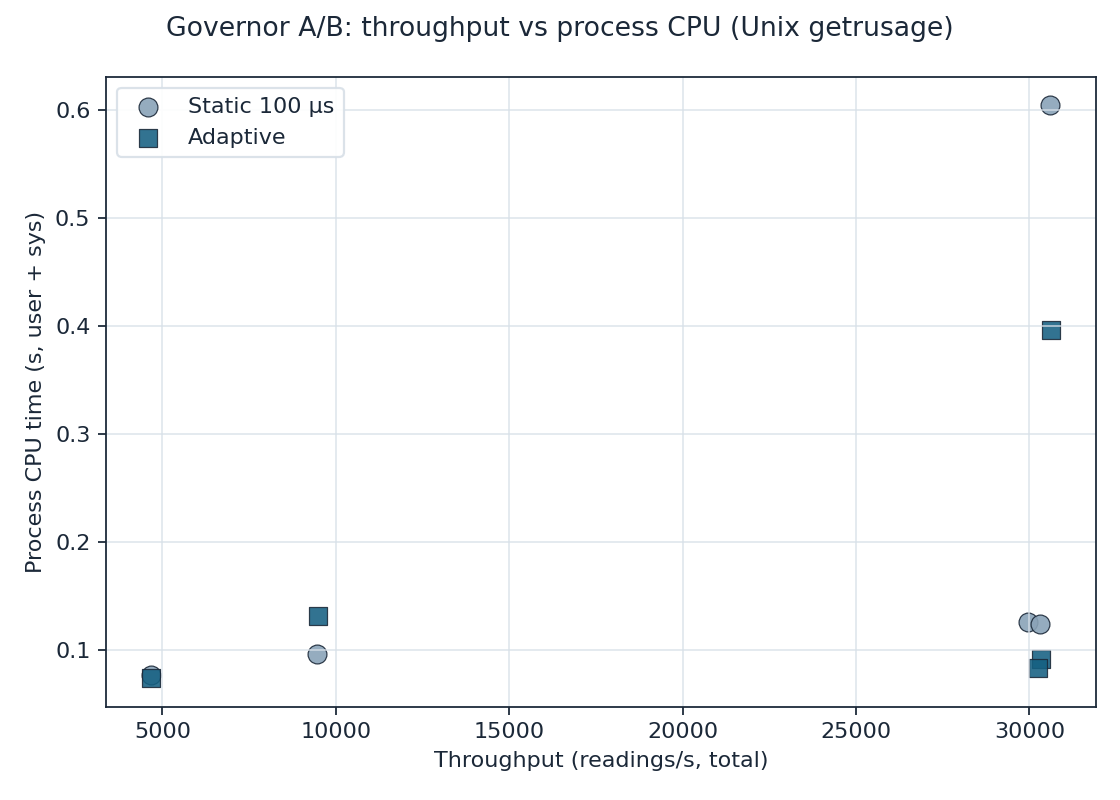
\includegraphics[width=\linewidth]{figures/governor_cpu_efficiency.png}
\caption{Governor A/B micro-bench: throughput versus process CPU seconds (\texttt{getrusage}).}
\label{fig:governor-cpu}
\end{figure}

\subsection*{Experiment D: load-scaling view}
The final experiment varies offered rate from 5000 to 40{,}000 readings per second per sensor while keeping queue capacity fixed at 256 and reader sleep at 0. Under zero consumer work, service rate scales smoothly from about 7.8k to 56.5k readings per second with zero upstream overwrites across all tested points. Under 200 $\mu$s consumer work, service rate saturates near 3.9k--4.2k readings per second while overwrite count rises rapidly from 11{,}263 at rate 5000 to 158{,}101 at rate 40{,}000. Figure~\ref{fig:load-scaling} shows the sharp separation between stable and overloaded operating regions.

\begin{figure}[H]
\centering
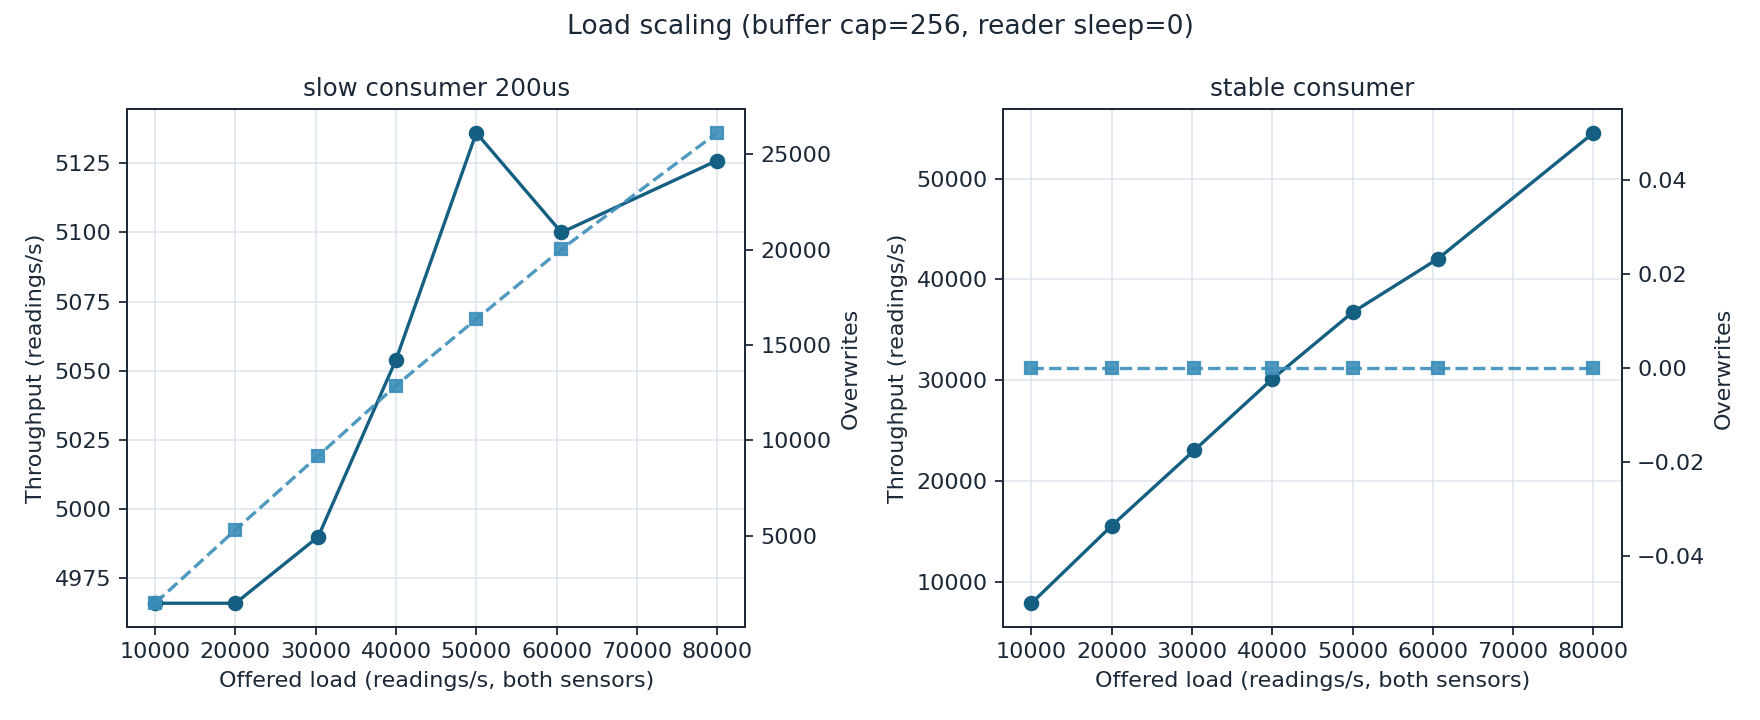
\includegraphics[width=\linewidth]{figures/load_scaling.png}
\caption{Load scaling under stable and overloaded consumer configurations.}
\label{fig:load-scaling}
\end{figure}

\section{Discussion}
\subsection*{Lazy-propagated segment trees and dynamic arrays (why not)}
If the student buffer were sharded into many fixed-size segments, a natural bookkeeping layer would be a \emph{dynamic array} of chunks plus a \emph{lazy-propagated segment tree} over chunk indices: range aggregates (occupancy, utilization, time coverage) update in \(O(\log N)\) while lazy tags defer work until queries force pushes to children. That pattern fits competitive programming and some analytics engines where thousands of shards justify the metadata machinery.

This project does not use it. At coursework scale the ingestion path is a single \texttt{VecDeque} under one monitor: \texttt{len}, high-water marks, and push/pop wait counters already expose the quantities a segment tree would summarize, without extra pointers, cache misses, or lazy invariants that must stay correct under concurrent chunk allocation. Sharding would also complicate the rubric story---condition synchronization and shutdown---without changing the queueing limits Section~\ref{sec:benchmark} already exhibits when \(\hat{\rho}>1\). The tree is asymptotically neat on paper; here it would mostly add debugging surface and obscure the OS teaching point (bounded buffer, backpressure, happens-before) in exchange for throughput headroom the workload does not need.

\subsection*{Persistence throughput and the single-writer trade-off}
Synchronous single-writer publication with explicit ACK preserves \textbf{coherent, torn-read-free} JSON for graders and dashboards, but it is deliberately a \textbf{serializing stage}: the aggregation consumer waits for durable commit before accepting the next frame. High-throughput systems therefore move durability \emph{off the critical path} using patterns this codebase does not implement: \emph{group commit} (amortize \texttt{fsync} across many logical records), \emph{double buffering} (one buffer being flushed while another accepts writes), \emph{write-behind} with a visible ``committed up to sequence $k$'' watermark, or \emph{asynchronous I/O} with ordered completion callbacks. Each option relaxes some aspect of the current ``every frame is immediately visible'' contract. For COMP2432 the strict stage is kept to make backpressure and failure modes legible; architectural discussion acknowledges where a production deployment would re-balance latency versus durability \cite{kleppmann2017}.

\subsection*{Compositional correctness }
The strongest alignment between this codebase and an operating-systems reading of Project Azure is not a fancier indexing structure but \textbf{contracts that span stages}: window rotation is \emph{fail-closed} (no partial frame is published if a worker is missing), the aggregation consumer waits for an explicit acknowledgement from the storage worker before treating a frame as drained, and dashboard-visible JSON is published only via \texttt{write-then-rename}. Together these rules make cross-thread and cross-file behavior inspectable: torn reads, silent drops on a full downstream queue, and ``almost correct'' statistics are ruled out by construction rather than by hope. That compositional discipline matches how OS courses want students to state invariants that outlive any single lock critical section.

\section{Conclusion and Future Work}
This submission addresses the COMP2432 Project Azure brief end-to-end. Buffer management is covered by per-sensor reader threads that use only the public \texttt{Sensor} trait, a bounded \texttt{SensorBufferManager} with blocking and timed pops, utilization statistics, and clean shutdown. The aggregation engine implements time windows, concurrent workers, merged statistics (Chan/Welford), anomaly flags, and storage hand-off with a barrier so partial windows are not published. Data storage serializes writes through one worker, flushes and rotates files, and publishes dashboard-visible JSON via write-then-rename so readers never see half-written snapshots. The web layer serves JSON on the required-style routes from those committed artifacts. Code quality is supported by modular crates, tests under \texttt{cargo test}, and reproducible benchmarks. Advanced work is represented by the adaptive polling governor, an extended benchmark suite, and evaluation that reports negative as well as positive results where appropriate.

Objectives from the specification are met in a traceable way: readers prevent simulated sensor overflow under tested loads; the student queue enforces backpressure; aggregation and persistence coordinate without data races on shared files; HTTP clients can query latest, aggregate, and per-sensor views. Correctness is argued through explicit invariants (drain-first ingestion, fail-closed windows, single-writer publication) rather than through informal claims.

Limitations remain. Anomaly detection is intentionally simple (windowed z-score only); the dashboard does not stream live updates; storage rewrites hourly JSONL for simplicity rather than using a segmented append-only log with compaction. Future work could add \emph{drift-aware} monitors (e.g., ADWIN/CUSUM-style change detection on stream moments), lightweight \emph{state-space} or Kalman-style prediction of sensor baselines for residual-based alerts, dynamic worker pools, WebSocket or SSE updates, batched or group-commit persistence, stronger durability policies (fsync cadence, checksums), or a lock-free hot path for the bounded queue while preserving the same external semantics. Those directions would build on the same pipeline boundaries validated here.

Finally, the written evidence and the repository are kept aligned deliberately: every figure path exists under \texttt{docs/figures/}, benchmark tables cite files under \texttt{data/bench/}, and the appendix records the exact command lines used to regenerate them. That pairing is meant to satisfy both the report rubric and the expectation that a marker can verify claims without guesswork.

\appendix
\section{Reproducibility Notes}
The project was validated with \texttt{cargo test} and benchmarked through repository binaries under \texttt{gateway/src/bin/}. Figure assets are generated by \texttt{docs/make\_figures.py} and written to \texttt{docs/figures/} (pipeline, queue, benchmarks, and process diagrams: shutdown, governor modes, window rotation, atomic write, backpressure). Governor and Pareto artifacts are reproduced with \texttt{cargo run --release -p gateway --bin azure\_bench -- sweep-governor 1200} (overwrites \texttt{data/bench/governor\_pareto\_sweep.jsonl}, including per-run \texttt{process\_cpu\_secs}), then \texttt{python3 docs/make\_figures.py}. A low-pressure snapshot is \texttt{azure\_bench zero-loss 2200}.

\section{Artifact Map}
The code and evidence cited most directly in this report are:
\begin{itemize}
\item \texttt{gateway/src/main.rs}: orchestration, scheduler, shutdown, and runtime statistics snapshot.
\item \texttt{gateway/src/buffer.rs}: bounded queue implementation and queue metrics.
\item \texttt{gateway/src/governor.rs}: adaptive polling controller.
\item \texttt{gateway/src/aggregation.rs}: dispatcher/worker reduction and fail-closed collection.
\item \texttt{gateway/src/storage.rs}: single-writer persistence, atomic publication, and storage metrics.
\item \texttt{data/bench/*.json*}: benchmark evidence used in the tables and figures.
\end{itemize}

\section{Submission Readiness}
At the time of writing, the repository contains all assets referenced by the main text: the benchmark JSON/JSONL files, generated figure PNG files, and the code paths discussed in the implementation section. The remaining manual step on this machine is PDF compilation, which depends on a local LaTeX toolchain being available.

\begin{thebibliography}{99}
\bibitem{silberschatz2018}
Silberschatz, A., Galvin, P. B., \& Gagne, G. (2018). \emph{Operating system concepts} (10th ed.). Wiley.

\bibitem{tanenbaum2014}
Tanenbaum, A. S., \& Bos, H. (2014). \emph{Modern operating systems} (4th ed.). Pearson.

\bibitem{andrews2000}
Andrews, G. R. (2000). \emph{Foundations of multithreaded, parallel, and distributed programming}. Addison-Wesley.

\bibitem{hoare1974}
Hoare, C. A. R. (1974). Monitors: An operating system structuring concept. \emph{Communications of the ACM}, \emph{17}(10), 549--557. \url{https://doi.org/10.1145/355620.361161}

\bibitem{dijkstra1968}
Dijkstra, E. W. (1968). Cooperating sequential processes. In F. Genuys (Ed.), \emph{Programming languages} (pp.~43--112). Academic Press.

\bibitem{little1961}
Little, J. D. C. (1961). A proof for the queueing formula \(L=\lambda W\). \emph{Operations Research}, \emph{9}(3), 383--387. \url{https://doi.org/10.1287/opre.9.3.383}

\bibitem{kleinrock1975}
Kleinrock, L. (1975). \emph{Queueing systems: Volume 1: Theory}. Wiley.

\bibitem{leboudec2001}
Le Boudec, J.-Y., \& Thiran, P. (2001). \emph{Network calculus: A theory of deterministic queuing systems for the internet}. Springer. \url{https://doi.org/10.1007/3-540-45318-7}

\bibitem{welford1962}
Welford, B. P. (1962). Note on a method for calculating corrected sums of squares and products. \emph{Technometrics}, \emph{4}(3), 419--420. \url{https://doi.org/10.2307/1266577}

\bibitem{chan1979}
Chan, T. F., Golub, G. H., \& LeVeque, R. J. (1979). Updating formulae and a pairwise algorithm for computing sample variances (Technical Report No. STAN-CS-79-773). Stanford University, Department of Computer Science.

\bibitem{rustbook2019}
Klabnik, S., \& Nichols, C. (2023). \emph{The Rust programming language} (2nd ed.). No Starch Press.

\bibitem{ruststd2026}
The Rust Project. (n.d.). \emph{The Rust standard library} [Computer software documentation]. Retrieved March 26, 2026, from \url{https://doc.rust-lang.org/std/}

\bibitem{bos2023}
Bos, M. (2023). \emph{Rust atomics and locks: Low-level concurrency in practice}. O'Reilly Media.

\bibitem{fielding2022}
Fielding, R., Nottingham, M., \& Reschke, J. (2022). \emph{HTTP semantics} (RFC 9110). Internet Engineering Task Force. \url{https://doi.org/10.17487/RFC9110}

\bibitem{tokio2026}
Tokio Contributors. (n.d.). \emph{Tokio: Asynchronous runtime for Rust} [Computer software documentation]. Retrieved March 26, 2026, from \url{https://docs.rs/tokio/}

\bibitem{crossbeam2026}
Crossbeam Contributors. (n.d.). \emph{Crossbeam: Tools for concurrent programming in Rust} [Computer software documentation]. Retrieved March 26, 2026, from \url{https://docs.rs/crossbeam/}

\bibitem{goetz2006}
Goetz, B., Peierls, T., Bloch, J., Bowbeer, J., Holmes, D., \& Lea, D. (2006). \emph{Java concurrency in practice}. Addison-Wesley.

\bibitem{dean2013}
Dean, J., \& Barroso, L. A. (2013). The tail at scale. \emph{Communications of the ACM}, \emph{56}(2), 74--80. \url{https://doi.org/10.1145/2408776.2408794}

\bibitem{sutter2005}
Sutter, H., \& Larus, J. (2005). Software and the concurrency revolution. \emph{ACM Queue}, \emph{3}(7), 54--62.

\bibitem{kleppmann2017}
Kleppmann, M. (2017). \emph{Designing data-intensive applications: The big ideas behind reliable, scalable, and maintainable systems}. O'Reilly Media.

\bibitem{ousterhout2018}
Ousterhout, J. K. (2018). \emph{A philosophy of software design}. Yaknyam Press.

\bibitem{lampson1980}
Lampson, B. W., \& Redell, D. D. (1980). Experience with processes and monitors in Mesa. \emph{Communications of the ACM}, \emph{23}(2), 105--117. \url{https://doi.org/10.1145/358818.358824}
\end{thebibliography}

\end{document}